\documentclass{article}
\usepackage{graphicx} % Required for inserting images
\graphicspath{{Images/}}
\usepackage[utf8]{inputenc}
\usepackage{multicol}
\usepackage{amsthm}
\usepackage{amsmath}
\usepackage{amsfonts}
\usepackage{xcolor}

\title{Analyse I - Integration Tricks from CMS (ily Dubuis)}
\author{Laura Paraboschi}
\date{BA1 - Automne 2023}

\begin{document}

\maketitle

\section{Somme de Riemann}
\begin{enumerate}
    \item On construit une partition de l'intervalle [a, b] en n sous-intervalles [$x_{k-1}$, $x_k$] avec 1 $\leq$ k $\leq$ n \\
    a = $x_0 < x_1 < $...$ < x_n$ = b
    \item Dans chaque intervalle [$x_{k-1}$, $x_k$], on choisit $t_k \in$ [$x_{k-1}$, $x_k$]
    \item On construit des rectangles de base $x_k - x_{k-1}$ et de hauteur f($t_k$)
    \item On calcule l'aire des rectangls $\sum_{k = 1}^{n} f(t_k)(x_k - x_{k-1})$
\end{enumerate}
\begin{figure}[htp]
    \centering
    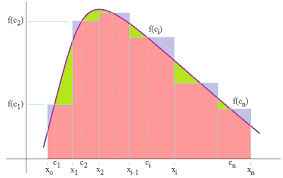
\includegraphics[width=8cm]{Images/riemann.png}
    \label{fig:enter-label}
\end{figure}
\subsection{Somme de Darboux}
Les sommes de Darboux sont les sommes de Riemann avec des $t_k$ particuliers :
\begin{itemize}
    \item Somme de Darboux inférieure : $t_k$ = $x_{k-1}$
    \item Somme de Darboux supérieure : $t_k$ = $x_{k}$
\end{itemize}
Note : La limite quand n ($\Delta x_k$) tend vers l'infini de Darboux Sup et Inf est la même

\section{Méthode de calculs de primitives}
\subsection{Primitives connues}
\begin{itemize}
    \item $\int x^k dx = \frac{1}{k+1}x^{k+1} + C\;  \forall k \in \mathbb{R} \setminus\{-1\}$
    \item $\int \frac{1}{x} dx = \ln{|x|} + C\;  \forall x\in \mathbb{R}^*$
    \item $\int e^x dx = e^x + C$
    \item $\int a^x dx = \frac{a^x}{\ln{(a)}} + C\;  \forall a > 0, a \neq 1 $
    \item $\int sin(x) dx = -cos(x) + C$
    \item $\int cos(x) dx = sin(x) + C$
    \item $\int \frac{1}{cos^2(x)} dx = tan(x) + C$
    \item $\int \frac{1}{sin^2(x)} dx = -cot(x) + C$
    \item $\int \frac{1}{1 + x^2} dx = arctan(x) + C$
    \item $\int \frac{1}{\sqrt{1 - x^2}} dx = arcsin(x) + C$
    \item $\int \frac{-1}{\sqrt{1 - x^2}} dx = arccos(x) + C$
    \item $\int sinh(x) dx = cosh(x) + C$
    \item $\int cosh(x) dx = sinh(x) + C$
    \item $\int \frac{1}{cosh^2(x)} dx = tanh(x) + C$
    \item $\int \frac{1}{sinh^2(x)} dx = -coth(x) + C$
    \item $\int \frac{1}{1 - x^2} dx = arctanh(x) + C$
\end{itemize}

\subsection{Méthodes basées sur l'observation}
\begin{itemize}
    \item On regarde si l'intégrant est, à une constante près, la dérivée d'une fonction connue\\
    ex : $\int \frac{1}{\sqrt{ax + b}}dx = \int \frac{2a}{2a\sqrt{ax + b}}dx =\frac{2}{a} \int (\sqrt{ax + b})'dx$
    \item On regarde si l'intégrant est la dérivée d'une fonction composée \\
    ex : f(x) = F(u(x) $\cdot$ u'(x)) = F(u(x))'
\end{itemize}

\subsection{Intégration par partie}
$\int u'vdx = uv - \int uv'dx$\\\\
Note : dessinez des flèches vers le haut et le bas pour ne pas se tromper sur quelle fonction intégrer et quelle fonction dériver\\
Note 2 : Ne pas hésiter à rajouter des termes annulant dans l'intégrale (1, $\frac{\sqrt{x}}{\sqrt{x}}$, ...) pour utiliser l'IPP\\
Note 3 : si l'intégrale tourne en boucle, essayer de retrouver l'intégrale de départ et résoudre une équation

\subsection{Intégration par changement de variable}
\begin{enumerate}
    \item On choisit une fonction $\phi \in C^1$ et bijective
    \item On pose x = $\phi(t)$
    \item On pose $\int f(x)dx = \int f(\phi(t))\cdot\phi'(t)dt$
\end{enumerate}
Astuce pour se rappeler de la formule :
\begin{enumerate}
    \item On pose x = $\phi(t)$
    \item On remplace dx par d$\phi(t) = \phi'(t) $
\end{enumerate}
\subsubsection{Quelques changements usuels}
\begin{itemize}
    \item Une fonction de la forme $\sqrt{1 - x^2}$ on peut poser :
    \begin{itemize}
        \item x = sin(t), t = arcsin(x), dx = cos(t)dt
        \item x = cos(t), t = arccos(x), dx = -sin(t)dt
    \end{itemize}
    \item Une fonction de la forme $\sqrt{1 + x^2}$ on peut poser :\\\\
    x = sinh(t), t = arcsinh(x), $\sqrt{1 + x^2}$ = cosh(t), dx = cosh(t)dt
    \item Une fonction de la forme $\sqrt{1 - x^2}$ on peut poser :
    \begin{itemize}
        \item x = cosh(t), pour x $\geq$ 1 et t $\geq$ 0, dx = sinh(t)dt, $\sqrt{1 - x^2}$ = sinh(t)
        \item x = -cosh(t), pour x $\leq$ -1 et t $\geq$ 0, dx = -sinh(t)dt, $\sqrt{1 - x^2}$ = sinh(t)
    \end{itemize}
\end{itemize}
\subsubsection{Primitiver des fonctions de la forme $\sqrt{P_2(x)}$ ($P_2(x) = ax^2 + bx + c$)}
\begin{itemize}
    \item $\Delta > 0, a < 0$ alors $\sqrt{P_2(x)}$ peut s'écrire sous la forme :\\
    $\lambda \sqrt{1 - z^2}$ pour z $\in $ [-1, 1]\\
    Dans ce cas on pose z = sin(t) ou z = cos(t)
    \item $\Delta < 0, a < 0$ alors $\sqrt{P_2(x)}$ peut s'écrire sous la forme :\\
    $\lambda \sqrt{1 + z^2}$\\
    Dans ce cas on pose z = sinh(t)
    \item $\Delta > 0, a > 0$ alors $\sqrt{P_2(x)}$ peut s'écrire sous la forme :\\
    $\lambda \sqrt{z^2 - 1}$\\
    Dans ce cas on pose z = cosh(t) si z $\geq$ 1 ou z = -cosh(t) si z $\leq$ -1
\end{itemize}
Exemple : $\sqrt{6x - x^2} \Rightarrow 6x - x^2 = -x^2 + 6x + 9 - 9 = -(x - 3)^2 + 9$\\
$\Rightarrow \sqrt{6x - x^2} = \sqrt{-(x - 3)^2 + 9} = 3\sqrt{1 - (\frac{x-3}{3})^2}$\\
On pose z = $\frac{x-3}{3} \Rightarrow 3\sqrt{1 - (\frac{x-3}{3})^2} = 3\sqrt{1 - z^2}$ 

\subsection{Intégration de fonctions rationnelles $\frac{P(x)}{Q(x)}$}
\begin{enumerate}
    \item Si degré P $>$ degré Q, alors diviser P par Q, $\frac{P(x)}{Q(x)} = S(x) + \frac{R(x)}{Q(x)}$
    \item Réécrire comme une somme de fractions simples
\end{enumerate}
Ces fractions simples sont appelées éléments simples, qui peuvent être de 2 espèces différentes :
\begin{itemize}
    \item 1ère espèce : $\frac{A}{(x-\alpha)^n}$
    \item 2ème espèce : $\frac{Bx + C}{(x^2 + bx + c)^n}$
\end{itemize}
Pour chaque polynômes de Q(x), le réécrire sous la forme d'un élément simple, autant de fois que son degré, et en augmentant la puissance à chaque fois.\\ Ex : $\frac{P(x)}{(x+2)^3} = \frac{A}{(x+2)} + \frac{B}{(x+2)^2} + \frac{C}{(x+2)^3}$ 
\subsubsection{Comment trouver efficacement A, B, C... ?}
\begin{itemize}
    \item Méthode par identification \\
    On remet les éléments simples sur le dénominateur de base, puis on égalise les numérateurs
    \item Méthode par évaluation \\
    On multiplie les deux côtés de notre équation par un polynome de x, puis on évalue x en un certain point. On peut aussi évaluer la limite en infini, ou simplement évaluer notre expression sur un x "gentil". Le but est d'éliminer des termes.
\end{itemize}
\subsubsection{Intégration des éléments simples}
\begin{itemize}
    \item Première espèce :
    \begin{itemize}
        \item $\int \frac{a}{x-\alpha}dx = aln(|x-\alpha|) + C$
        \item$\int \frac{a}{(x-\alpha)^2}dx = \frac{-a}{x-\alpha} + C$
        \item $\int \frac{a}{(x-\alpha)^n}dx =\frac{-a}{n-1} \cdot \frac{1}{(x-\alpha)^{n-1}} + C$ avec n $\geq$ 2
    \end{itemize}
    \item Deuxième espèce (formule pas cool) : \\
    $\int \frac{px + q}{x^2 + bx + c}dx = \frac{p}{2}ln|x^2 + bx + c| + \frac{q - \frac{bp}{2}}{c - (\frac{b}{2})^2} \sqrt{c - (\frac{b}{2})^2}arctan(\frac{x + \frac{b}{2}}{\sqrt{c - (\frac{b}{2})^2}}) + C $
\end{itemize}
Exemple 2ème espèce : \\\\
$\int \frac{7x + 5}{x^2 + 2x + 5}dx = \frac{7}{2}\int \frac{2x + \frac{10}{7}}{x^2 + 2x + 5}dx = \frac{7}{2}\int \frac{2x + 2 \frac{10}{7} - 2}{x^2 + 2x + 5}dx\\\\ = \frac{7}{2}\int \frac{2x + 2}{x^2 + 2x + 5}dx - 2 \int \frac{1}{x^2 + 2x + 1 + 4}dx = \frac{7}{2}ln|x^2 + 2x + 5| - 2 \int \frac{1}{(x+1)^2 + 4}dx\\\\ =  \frac{7}{2}ln|x^2 + 2x + 5| - \frac{1}{2} \int \frac{1}{(\frac{(x+1)}{2})^2 + 1}dx = \frac{7}{2}ln|x^2 + 2x + 5| - \frac{1}{2} arctan(\frac{x+1}{2}) + C$

\subsection{Intégration de fonctions rationnelles trigonométriques (f(x) = $\frac{P(cos(x), sin(x))}{Q(cos(x), sin(x))}$)}
Le principe est d'utiliser les Tests de Bioche :
\begin{enumerate}
    \item Si $f(\pi - x)d(\pi - x) = f(x)dx$, on pose z = sin(x)
    \item Si $f(-x)d(-x) = f(x)dx$, on pose z = cos(x)
    \item Si $f(\pi  + x)d(\pi + x) = f(x)dx$, on pose z = tan(x)
    \item Si aucun test ne marche, on pose z = tan($\frac{x}{2}$)
\end{enumerate}
Astuce : utiliser les identités trigonométriques des angles doubles pour passer de tan(x) à sin(x)/cos(x) :
\begin{itemize}
    \item cos(2x) = $\frac{1 - tan^2(x)}{1 + tan^2(x)}$
    \item sin(2x) = $\frac{2tan(x)}{1 + tan^2(x)}$
\end{itemize}
Astuce 2 : Changement pour t = tan($\frac{x}{2}$)
\begin{itemize}
    \item cos(x) = $\frac{1 - t^2}{1 + t^2}$
    \item sin(x) = $\frac{2t}{1 + t^2}$
    \item tan(x) = $\frac{2t}{1 - t^2}$
\end{itemize}
\end{document}